\documentclass[10pt]{beamer}

\usetheme{metropolis}
\usepackage{appendixnumberbeamer}

\usepackage{booktabs}
\usepackage[scale=2]{ccicons}

\usepackage{pgfplots}
\usepgfplotslibrary{dateplot}

\usepackage{xspace}
\newcommand{\themename}{\textbf{\textsc{metropolis}}\xspace}

\title{RoboCup - System}
%\subtitle{A modern beamer theme}
\date{October 26, 2017}
\author{Florian Lier \& Johannes Kummert \& Dominik Sixt}
%\institute{Center for modern beamer themes}
%\titlegraphic{\hfill
\includegraphics[height=1.5cm]{logo.pdf}}
\titlegraphic{\hfill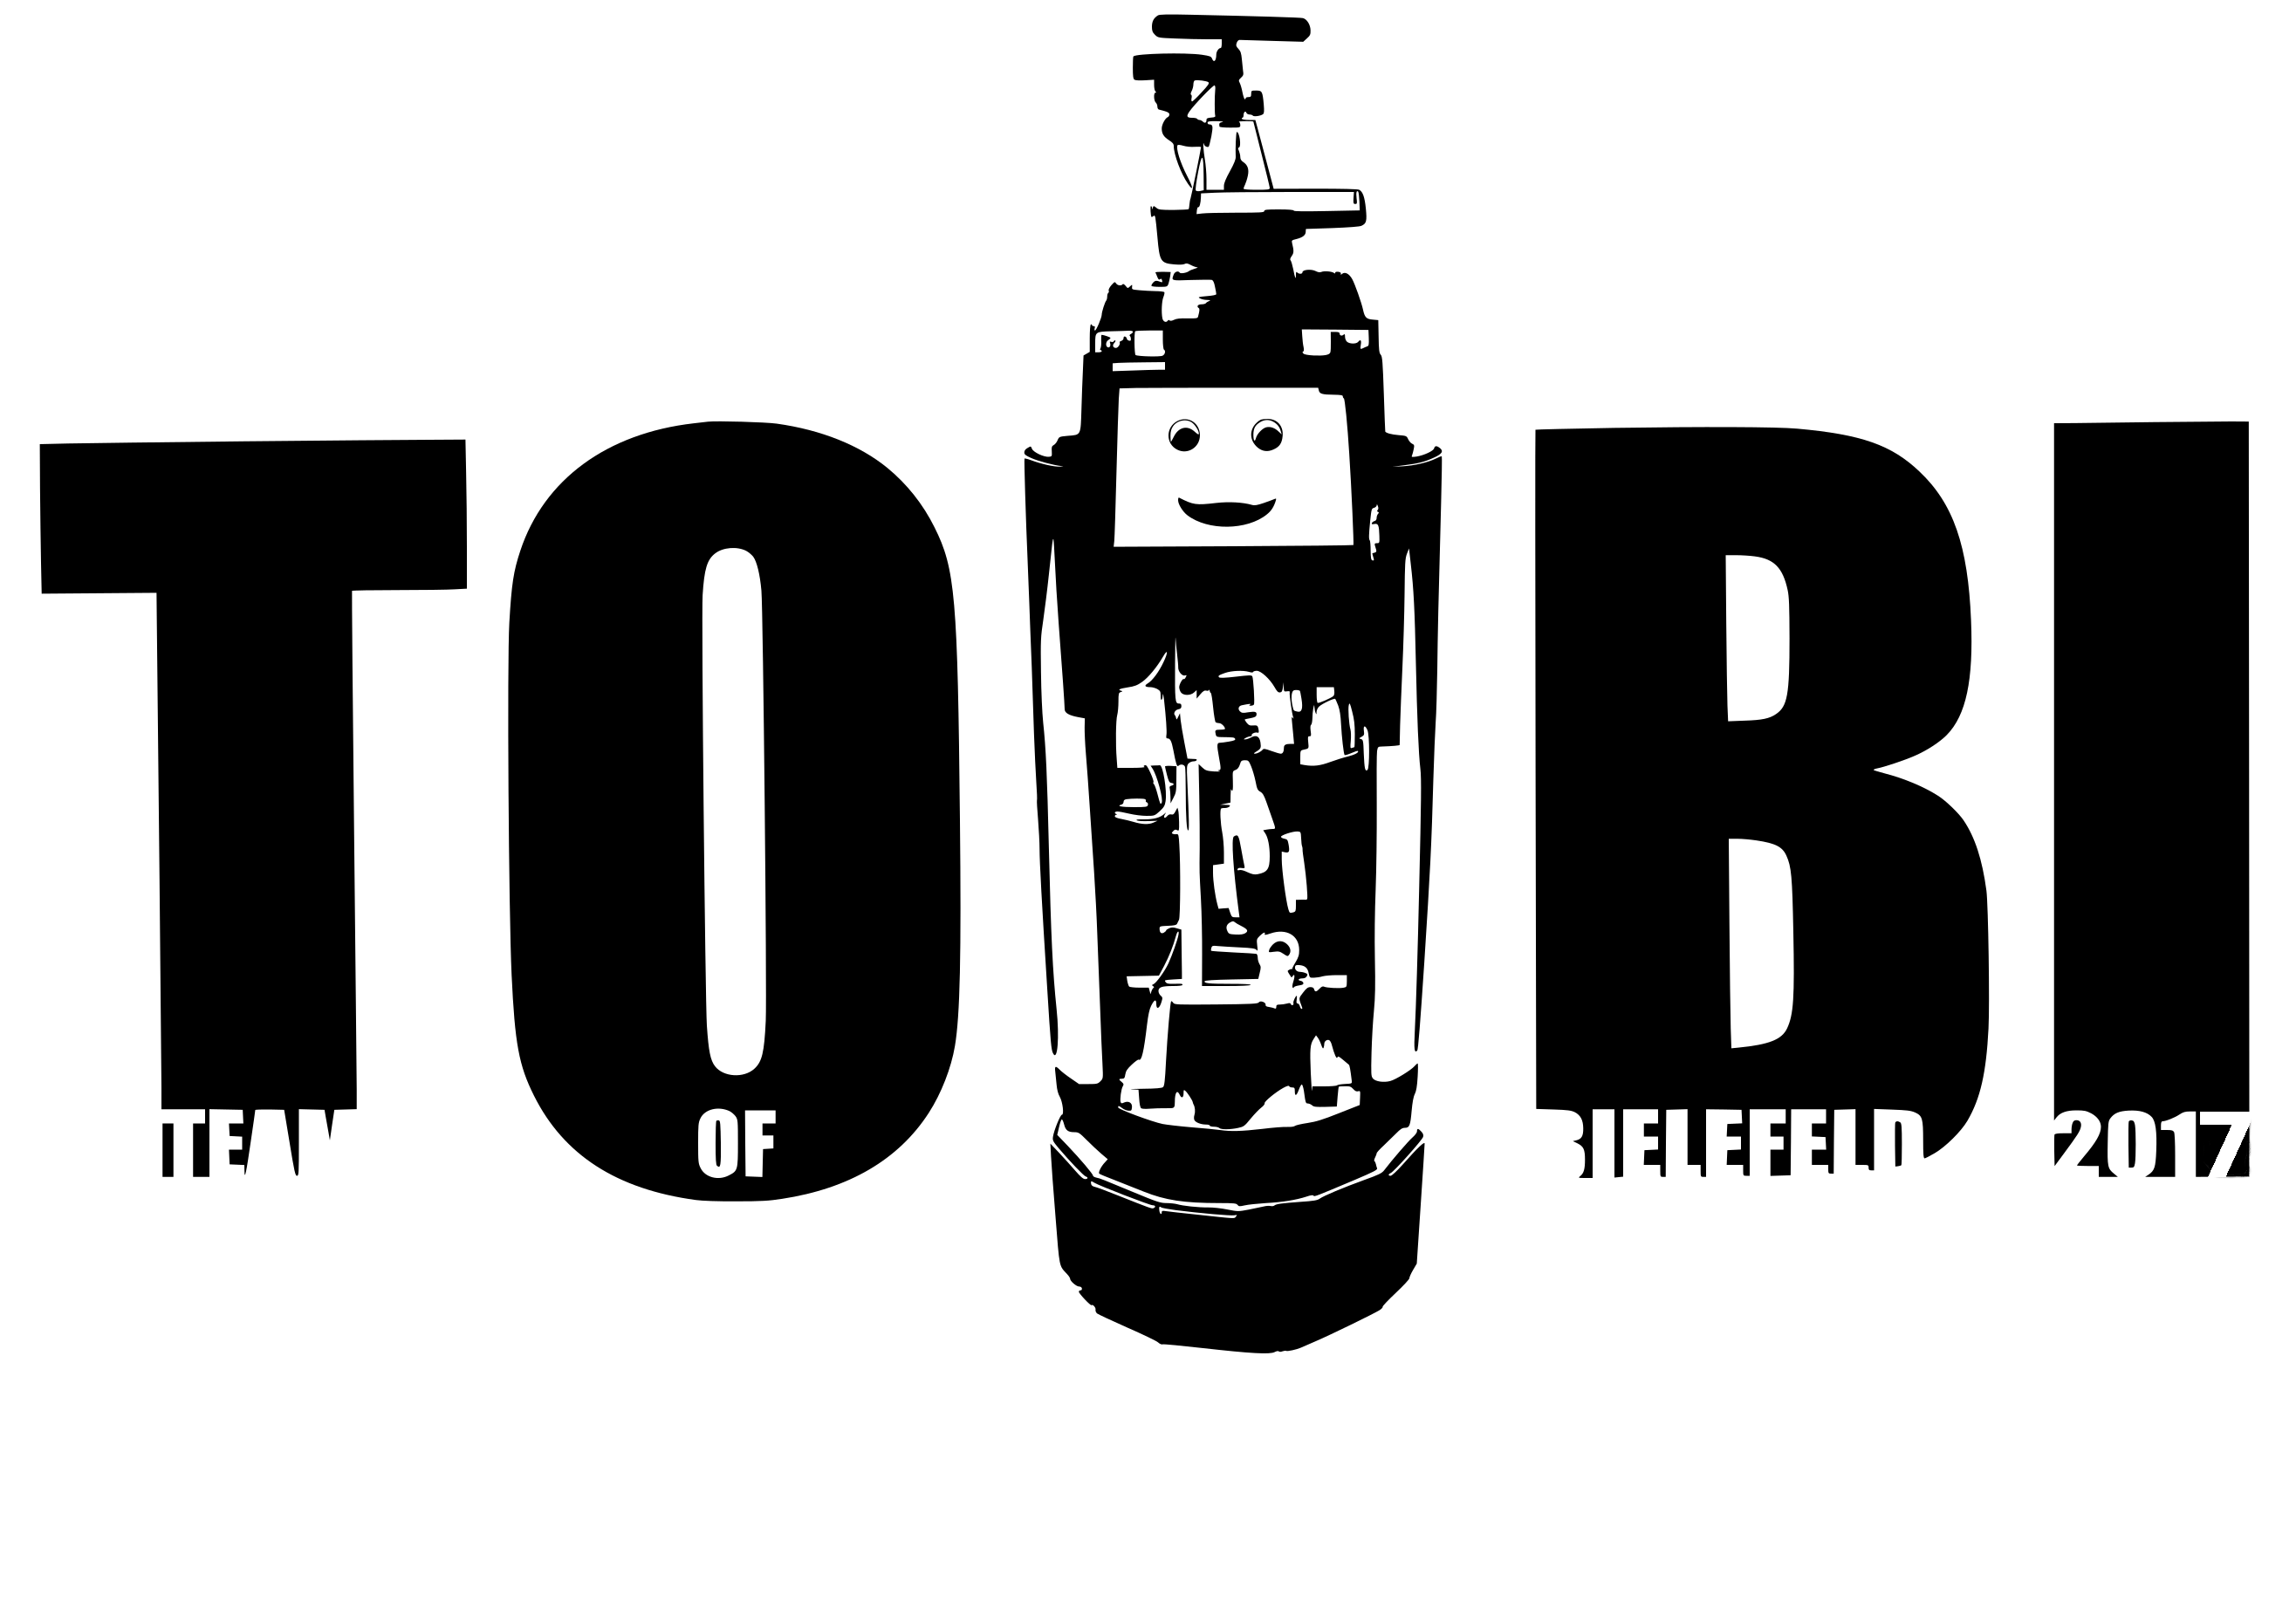
\includegraphics[height=1.5cm]{tobi_logo.png}}

\begin{document}

\maketitle

\begin{frame}{Table of contents}
  \setbeamertemplate{section in toc}[sections numbered]
  \tableofcontents[hideallsubsections]
\end{frame}

\section{Cognitive Interaction Toolkit}

\section{vDemo}

\section{BonSAI} % ... Sensor Actuator Interface
\begin{frame}[fragile]{BonSAI - Motivation}
	
	\begin{itemize}
		\item multiple software components
		\item perception and interpretation
		\item complex scenarios
		\item component agnostic
		\item robot agnostic
	\end{itemize}
	
\end{frame}

\begin{frame}[fragile]{BonSAI - Layers}

	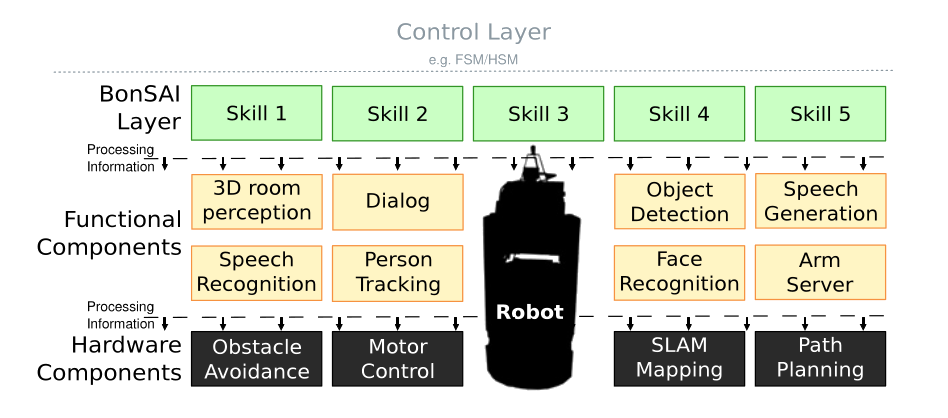
\includegraphics[scale=0.35]{bonsai_layerCut}

\end{frame}

\begin{frame}[fragile]{BonSAI - Structure}
	
	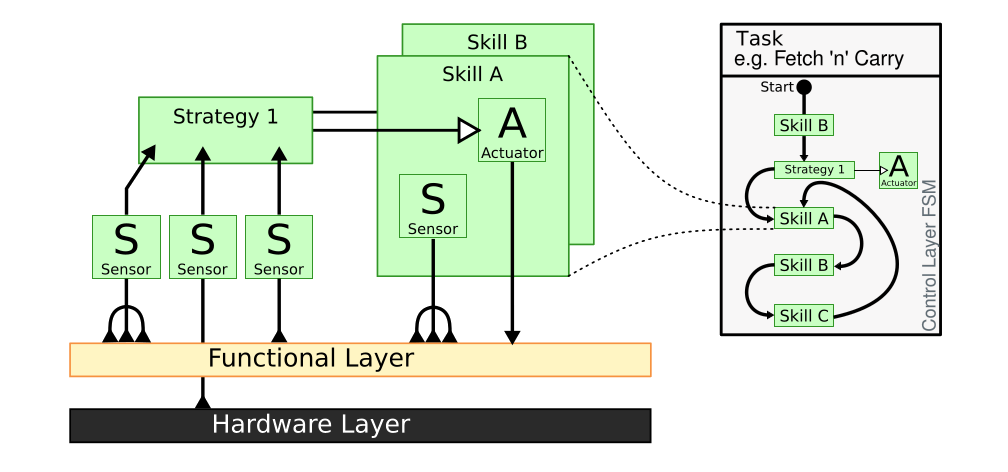
\includegraphics[scale=0.32]{bonsai_usageCut}
	
\end{frame}

\begin{frame}[fragile]{BonSAI - Example}
	
	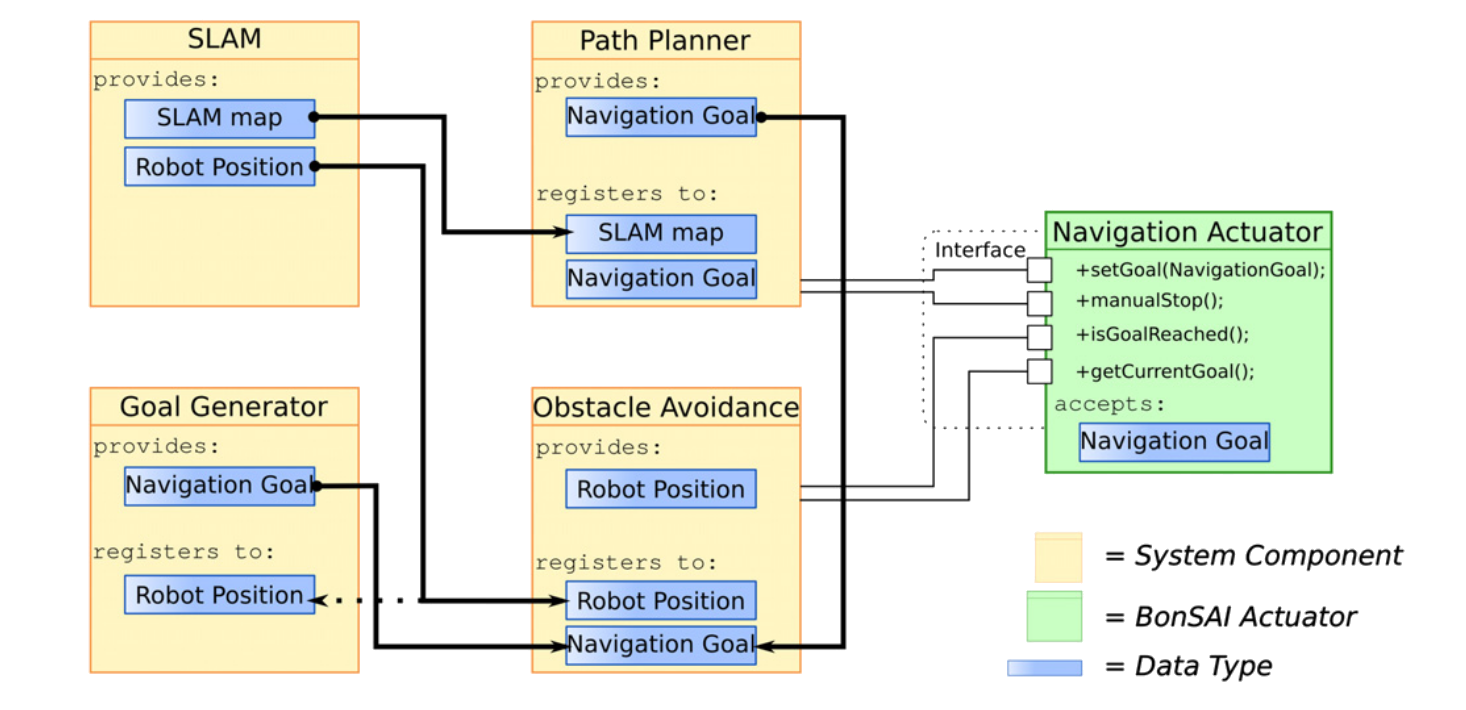
\includegraphics[scale=0.23]{bonsai_navCut}
	
\end{frame}

\begin{frame}[fragile]{Metropolis}

  The \themename theme is a Beamer theme with minimal visual noise
  inspired by the \href{https://github.com/hsrmbeamertheme/hsrmbeamertheme}{\textsc{hsrm} Beamer
  Theme} by Benjamin Weiss.

  Enable the theme by loading

  \begin{verbatim}    \documentclass{beamer}
    \usetheme{metropolis}\end{verbatim}

  Note, that you have to have Mozilla's \emph{Fira Sans} font and XeTeX
  installed to enjoy this wonderful typography.
\end{frame}


\begin{frame}[allowframebreaks]{References}

  \bibliography{demo}
  \bibliographystyle{abbrv}

\end{frame}

\end{document}
